\chapter{R-Trees as a database level Nearest Neighbours Algorithm}

In MoodCat, the core function of the rooms is to find songs that fit to your mood. Finding these songs should be autonomous and accurate. In our development we opted to achieve this using a K-Nearest Neighbour (KNN) algorithm.

Such an algorithm finds the K nearest elements from a given point. Consider the room to be a point in 2D space (x axis is the valence vale, the y axis is the arousal value). For example, take the graphic below. The red dot is the room we're finding a song for, the green and blue dots are songs defined with a VA-Vector. The purple circle describes a KNN with K = 3, while the blue circle describes a KNN with K = 7. \\
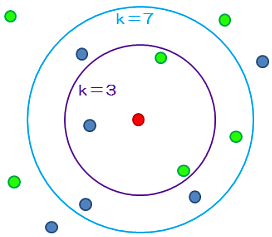
\includegraphics[scale=0.6]{knearestneighboursexample.png}\\

In developing MoodCat, we found our initial, naive implementation to slow down drastically with a high amount of songs and rooms. A solution had to be found. Initially, we created an Approximate Nearest Neighbours (ANN) implementation using a KD-tree. This remedies the slow runtime by calculating an approximate subset of points "sort of close" to the room. On this subset our original NN algorithm could run. Having solved the runtime complexity issues, we ran into memory issues instead. Indexing all songs in a KD-tree still requires every song object to be loaded into memory. We needed to find a sure-fire, effecient way of finding appropriate songs for a room.\\

We found the answer in the most unexpected part of the application: The database. Specifically an R-tree index. R-trees were proposed in 1984 by Antonin Guttman\footnote{http://www-db.deis.unibo.it/courses/SI-LS/papers/Gut84.pdf}. 